\subsection*{Tuần 2}

\subsubsection*{2.1 Mô tả công việc}
Trong tuần thứ hai, sinh viên được hướng dẫn nghiên cứu hồ sơ đề xuất kỹ thuật (Technical Proposal) nhằm tìm hiểu bài toán, mô hình tổng thể và kiến trúc giải pháp của dự án. Nội dung nghiên cứu tập trung vào việc xác định các thành phần chính của hệ thống, mối liên kết giữa các phân hệ nghiệp vụ và quy trình truyền dữ liệu từ thiết bị IoT đến hệ thống quản lý trung tâm.

Thông qua quá trình nghiên cứu tài liệu, sinh viên bước đầu hình thành cái nhìn tổng quan về kiến trúc hệ thống trước khi tham gia vào các công việc thiết kế và phát triển ở các tuần tiếp theo.

Các công việc chính được thực hiện trong tuần gồm:

\begin{itemize}
    \item Nghiên cứu hồ sơ đề xuất kỹ thuật của dự án.
    \item Tìm hiểu mô hình tổng thể của hệ thống.
    \item Tìm hiểu kiến trúc giải pháp ở mức tổng quan.
    \item Tìm hiểu các thành phần chính và vai trò của từng thành phần.
    \item Tìm hiểu quy trình nghiệp vụ và luồng dữ liệu trong hệ thống.
    \item Xác định phạm vi công việc sẽ thực hiện trong giai đoạn phát triển.
\end{itemize}

\subsubsection*{2.2 Nghiên cứu hồ sơ đề xuất kĩ thuật}

\textbf{Bối cảnh:}

Theo hồ sơ đề xuất kỹ thuật mà công ty cung cấp, khách hàng đang chuyển đổi từ mô hình kinh doanh bán máy lọc nước truyền thống sang mô hình cung cấp dịch vụ cho thuê kết hợp bảo trì định kỳ. Mô hình này hướng đến việc tạo nguồn doanh thu định kỳ, nâng cao chất lượng dịch vụ sau bán hàng và xây dựng nền tảng quản lý có khả năng mở rộng khi số lượng khách hàng và thiết bị ngày càng tăng.

Qua nghiên cứu tài liệu, em nhận thấy hệ thống không chỉ phục vụ quản lý thông tin khách hàng và hợp đồng mà còn tích hợp giải pháp IoT nhằm thu thập dữ liệu vận hành của máy lọc nước. Việc kết hợp giữa dữ liệu nghiệp vụ và dữ liệu từ thiết bị giúp doanh nghiệp có thể theo dõi trạng thái hoạt động của từng máy, phát hiện bất thường và hỗ trợ xây dựng kế hoạch bảo trì chủ động thay vì chỉ xử lý khi xảy ra sự cố.

Trong phạm vi thực tập, việc nghiên cứu hồ sơ đề xuất kỹ thuật giúp em hiểu được kiến trúc tổng thể của hệ thống cũng như mối liên hệ giữa phần cứng IoT, hệ thống backend và phần mềm quản lý. Đây là nền tảng quan trọng trước khi triển khai các công việc như thiết kế phần cứng sử dụng ESP32, xây dựng hệ thống tiếp nhận dữ liệu MQTT và phát triển website quản lý.

Vì đây chỉ là hồ sơ đề xuất kĩ thuật tạm thời, chưa phải là giải pháp toàn diện cho hệ thống, nên trong quá trình thực hiện sẽ có sự thay đổi khi sinh viên triển khai giải pháp.

% \textbf{Khách hàng vì còn eo hẹp kinh phí nên kèo này chưa chốt.}

\subsubsubsection*{Mục tiêu nghiên cứu}

Mục tiêu của tuần này là tìm hiểu bài toán và phạm vi của dự án thông qua hồ sơ đề xuất kỹ thuật. Các nội dung nghiên cứu tập trung vào:

\begin{itemize}
    \item Hiểu bài toán mà hệ thống cần giải quyết.
    \item Nắm được mô hình tổng thể của hệ thống.
    \item Xác định vai trò của các thành phần chính.
    \item Tìm hiểu quy trình nghiệp vụ của hệ thống.
    \item Nghiên cứu kiến trúc IoT và luồng dữ liệu tổng quát.
    \item Chuẩn bị kiến thức nền phục vụ cho các tuần phát triển tiếp theo.
\end{itemize}

\subsubsubsection*{Phạm vi nghiên cứu}

Trong tuần này, sinh viên chỉ dừng ở mức nghiên cứu và tìm hiểu kiến trúc tổng thể của hệ thống. Các nội dung như phân tích yêu cầu chi tiết, thiết kế cơ sở dữ liệu, thiết kế API, xây dựng backend, lập trình thiết bị và kiểm thử chưa được triển khai ở giai đoạn này.

Mục tiêu chính là hiểu được cách hệ thống được tổ chức, mối liên hệ giữa các thành phần và vai trò của từng lớp trong kiến trúc tổng thể.

\subsubsection*{2.3 Mô hình tổng thể hệ thống}


Theo hồ sơ đề xuất kỹ thuật của công ty HPT, hệ thống được tổ chức thành ba nhóm chức năng chính gồm \textbf{Core System}, \textbf{Omnichannel Integration} và \textbf{Field Service \& IoT}. Mỗi nhóm đảm nhận một vai trò riêng nhưng được liên kết với nhau nhằm hình thành một hệ thống quản lý thống nhất.

\begin{figure}[H!]
    \centering
    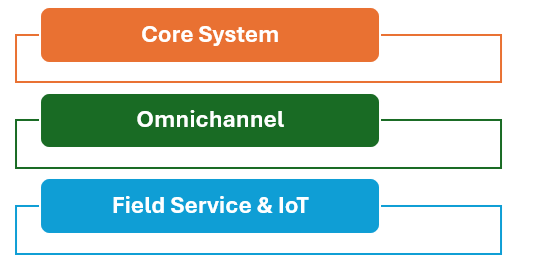
\includegraphics[width=0.5\textwidth]{include/image/kien_truc_tong_the.png}
    \caption{Kiến trúc tổng thể của hệ thống}
    \label{fig:overall_architecture}
\end{figure}

Trong đó:

\begin{itemize}
    \item Core System là trung tâm quản lý các nghiệp vụ như khách hàng, hợp đồng, thiết bị và bảo trì.
    \item Omnichannel Integration tiếp nhận và đồng bộ dữ liệu từ nhiều kênh tương tác với khách hàng.
    \item Field Service \& IoT hỗ trợ hoạt động kỹ thuật tại hiện trường và thu thập dữ liệu từ các thiết bị IoT.
\end{itemize}

Qua nghiên cứu mô hình tổng thể, em nhận thấy kiến trúc được thiết kế theo hướng phân tách chức năng rõ ràng giữa các nhóm nghiệp vụ và hệ thống thu thập dữ liệu. Cách tổ chức này giúp từng thành phần có thể phát triển tương đối độc lập nhưng vẫn đảm bảo khả năng trao đổi dữ liệu thông qua các cơ chế tích hợp chung. Đồng thời, việc phân chia thành nhiều lớp chức năng cũng tạo điều kiện mở rộng hệ thống khi số lượng thiết bị hoặc người dùng tăng lên trong tương lai.

\subsubsection*{2.4 Core System}

\subsubsubsection*{Vai trò}

Core System là trung tâm xử lý nghiệp vụ của toàn bộ hệ thống. Theo hồ sơ đề xuất kỹ thuật, thành phần này quản lý các thông tin quan trọng như khách hàng, thiết bị, hợp đồng, thanh toán và bảo trì. Mọi dữ liệu từ các thành phần khác cuối cùng đều được đồng bộ về Core System nhằm đảm bảo tính nhất quán trong quá trình vận hành.

Đối với sinh viên thực tập, việc tìm hiểu Core System giúp hình dung được nơi dữ liệu IoT sẽ được tích hợp và khai thác trong các chức năng quản lý sau này, thay vì chỉ xem hệ thống IoT như một thành phần hoạt động độc lập.

\subsubsubsection*{Các phân hệ chính}

Theo hồ sơ đề xuất kỹ thuật, Core System bao gồm các phân hệ chính như CRM, Asset Management, Contract Management, Billing System và Maintenance Management. Mỗi phân hệ đảm nhiệm một chức năng nghiệp vụ riêng nhưng đều sử dụng chung dữ liệu của hệ thống.

Qua nghiên cứu tài liệu, em nhận thấy Asset Management giữ vai trò quan trọng trong bài toán quản lý máy lọc nước vì đây là nơi quản lý toàn bộ thông tin của từng thiết bị như mã định danh, vị trí lắp đặt, trạng thái hoạt động và lịch sử bảo trì. Điều này cho thấy dữ liệu thu thập từ hệ thống IoT không tồn tại độc lập mà được liên kết với từng thiết bị cụ thể trong cơ sở dữ liệu nghiệp vụ.

\subsubsubsection*{Mối liên kết giữa các phân hệ}

Các phân hệ trong Core System không hoạt động độc lập mà liên kết với nhau theo vòng đời của một dịch vụ. Thông tin khách hàng được liên kết với hợp đồng thuê, hợp đồng gắn với thiết bị được lắp đặt, đồng thời phát sinh hóa đơn định kỳ và lịch bảo trì trong suốt quá trình sử dụng.

Qua nghiên cứu hồ sơ đề xuất kỹ thuật, em nhận thấy cách tổ chức dữ liệu này giúp đảm bảo tính nhất quán giữa các nghiệp vụ và tạo nền tảng để tích hợp dữ liệu IoT vào quá trình quản lý. Khi thiết bị gửi dữ liệu vận hành về hệ thống, dữ liệu có thể được liên kết trực tiếp với khách hàng, hợp đồng và lịch sử bảo trì tương ứng, từ đó hỗ trợ theo dõi tình trạng thiết bị và nâng cao hiệu quả quản lý dịch vụ.
\subsubsection*{2.5 Omnichannel Integration}

\subsubsubsection*{Vai trò}

Theo hồ sơ đề xuất kỹ thuật, Omnichannel Integration là lớp trung gian giúp hệ thống tiếp nhận và đồng bộ dữ liệu từ nhiều kênh tương tác khác nhau như Website, Facebook, Zalo và Pancake. Các thông tin như khách hàng tiềm năng, yêu cầu tư vấn hoặc đơn hàng sẽ được tập trung về Core System để quản lý thống nhất.

Qua nghiên cứu tài liệu, em nhận thấy Omnichannel không phải là trọng tâm trong phạm vi thực tập nhưng đóng vai trò quan trọng trong việc đảm bảo dữ liệu khách hàng được quản lý tập trung thay vì phân tán trên nhiều nền tảng khác nhau. Điều này giúp các bộ phận kinh doanh, chăm sóc khách hàng và kỹ thuật có thể khai thác cùng một nguồn dữ liệu trong quá trình vận hành.

\subsubsubsection*{Nhận xét}

Mặc dù không trực tiếp tham gia phát triển các chức năng Omnichannel, việc tìm hiểu thành phần này giúp em hiểu được nguồn gốc của dữ liệu khách hàng trước khi được liên kết với thông tin thiết bị và dữ liệu IoT trong hệ thống quản lý.

\subsubsection*{2.6 Field Service \& IoT}

\subsubsubsection*{Vai trò của Field Service và IoT}

Theo hồ sơ đề xuất kỹ thuật, Field Service hỗ trợ kỹ thuật viên thực hiện các công việc ngoài hiện trường như tiếp nhận lịch bảo trì, check-in tại địa điểm lắp đặt, cập nhật trạng thái công việc và ghi nhận kết quả sau khi hoàn thành.

Bên cạnh đó, hệ thống IoT được tích hợp nhằm thu thập dữ liệu vận hành từ các máy lọc nước trong quá trình sử dụng. Dữ liệu này được sử dụng để theo dõi trạng thái thiết bị, phát hiện các dấu hiệu bất thường và hỗ trợ xây dựng kế hoạch bảo trì dựa trên tình trạng thực tế thay vì chỉ thực hiện bảo trì theo định kỳ.

Qua nghiên cứu hồ sơ đề xuất kỹ thuật, em nhận thấy IoT là thành phần tạo nên sự khác biệt của hệ thống. Nếu Core System tập trung quản lý thông tin nghiệp vụ thì IoT cung cấp dữ liệu vận hành thực tế từ thiết bị, giúp doanh nghiệp có thể theo dõi tình trạng máy lọc nước theo thời gian và nâng cao hiệu quả quản lý dịch vụ.

\subsubsubsection*{Kiến trúc IoT bốn lớp}

Hồ sơ đề xuất kỹ thuật mô tả hệ thống IoT theo mô hình bốn lớp gồm Perception Layer, Network Layer, Processing Layer và Application Layer. Qua nghiên cứu, em nhận thấy việc phân chia thành nhiều lớp giúp mỗi thành phần đảm nhận một chức năng riêng, đồng thời làm cho hệ thống dễ bảo trì và mở rộng hơn.

\begin{itemize}
    \item \textbf{Perception Layer}: là lớp thu thập dữ liệu từ các thiết bị và cảm biến được lắp đặt trên máy lọc nước. Trong dự án, ESP32 đóng vai trò là bộ điều khiển trung tâm, đọc dữ liệu từ các cảm biến như TDS, áp suất, lưu lượng nước và trạng thái lõi lọc trước khi gửi lên hệ thống. Đây là tầng quyết định chất lượng dữ liệu đầu vào của toàn bộ hệ thống.

    \item \textbf{Network Layer}: chịu trách nhiệm truyền dữ liệu từ thiết bị đến hệ thống thông qua các giao thức như MQTT hoặc HTTP sử dụng Wi-Fi hoặc mạng di động. Qua nghiên cứu tài liệu, em nhận thấy MQTT phù hợp với bài toán này nhờ cơ chế publish/subscribe, giúp giảm chi phí truyền dữ liệu và hỗ trợ nhiều thiết bị kết nối đồng thời.

    \item \textbf{Processing Layer}: tiếp nhận dữ liệu từ các thiết bị, thực hiện kiểm tra, chuẩn hóa, xử lý nghiệp vụ và lưu trữ vào cơ sở dữ liệu. Việc tách tầng xử lý khỏi thiết bị giúp giảm khối lượng tính toán trên ESP32, đồng thời tạo điều kiện bổ sung các chức năng phân tích hoặc cảnh báo mà không cần thay đổi chương trình trên thiết bị.

    \item \textbf{Application Layer}: cung cấp giao diện Web hoặc Dashboard để hiển thị dữ liệu, cảnh báo và trạng thái hoạt động của thiết bị. Theo em, việc tách riêng tầng hiển thị giúp giao diện người dùng có thể phát triển độc lập với hệ thống thu thập dữ liệu phía dưới.
\end{itemize}

\subsubsubsection*{Quy trình hệ thống giám sát máy lọc nước}

Theo mô hình được đề xuất trong hồ sơ kỹ thuật, dữ liệu được truyền từ thiết bị đến hệ thống quản lý thông qua giao thức MQTT và được xử lý theo các bước sau:

\begin{enumerate}
    \item ESP32 đọc dữ liệu từ các cảm biến như TDS, áp suất, lưu lượng nước và trạng thái hoạt động của máy lọc nước.
    \item Thiết bị kết nối Internet thông qua Wi-Fi hoặc 4G và gửi dữ liệu lên MQTT Broker (HiveMQ Cloud) theo topic được định danh cho từng thiết bị.
    \item Ứng dụng Device Service triển khai trên máy chủ sử dụng MQTT Client để subscribe các topic tương ứng và tiếp nhận dữ liệu từ Broker.
    \item Dữ liệu sau khi được kiểm tra và xử lý sẽ được lưu vào cơ sở dữ liệu Microsoft SQL Server.
    \item Dashboard truy xuất dữ liệu từ cơ sở dữ liệu để hiển thị trạng thái thiết bị, biểu đồ vận hành và các cảnh báo phục vụ công tác giám sát.
\end{enumerate}

\begin{figure}[H]
    \centering
    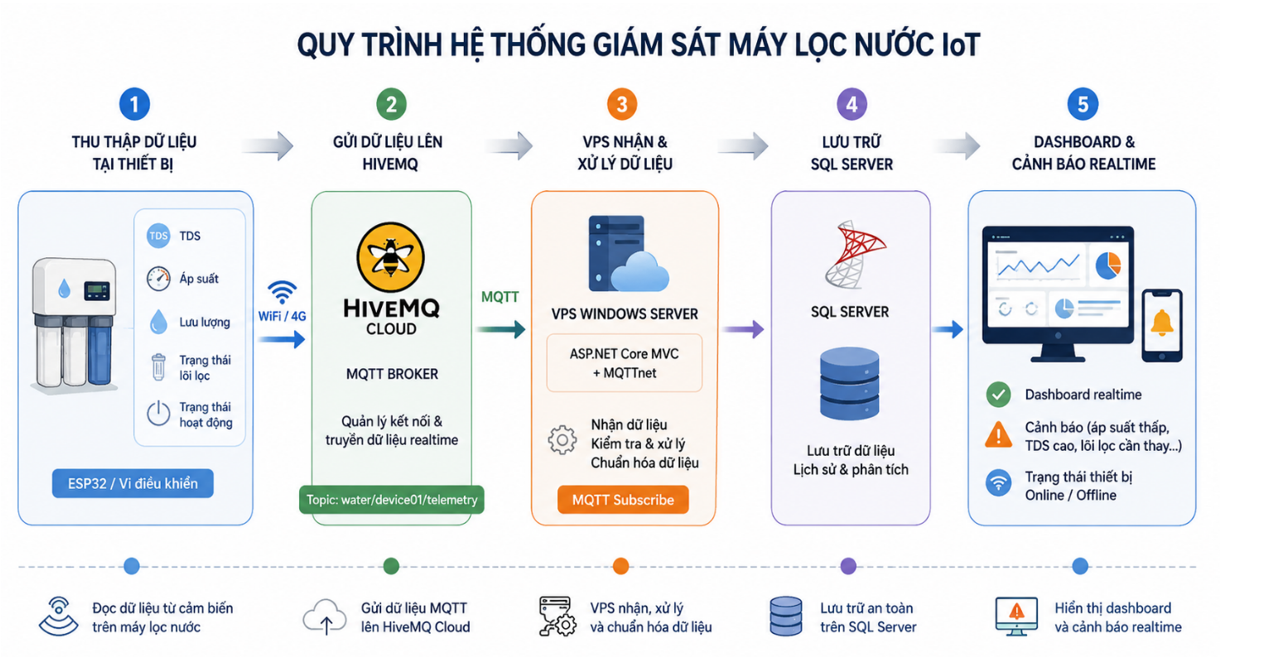
\includegraphics[width=0.9\textwidth]{include/image/quy_trinh_iot.png}
    \caption{Quy trình truyền dữ liệu IoT trong hệ thống}
    \label{fig:iot_process}
\end{figure}

\subsubsubsection*{Phân tích quy trình truyền dữ liệu}

Qua nghiên cứu hồ sơ đề xuất kỹ thuật, hệ thống sử dụng mô hình truyền thông theo cơ chế \textit{publish/subscribe}. Trong đó, ESP32 đóng vai trò \textit{Publisher}, HiveMQ Cloud là \textit{MQTT Broker} và ứng dụng Device Service trên máy chủ là \textit{Subscriber}.

Theo em, việc sử dụng Broker làm trung gian giúp thiết bị không cần kết nối trực tiếp với ứng dụng xử lý dữ liệu. Điều này làm giảm sự phụ thuộc giữa các thành phần trong hệ thống và giúp việc mở rộng số lượng thiết bị trở nên thuận lợi hơn. Khi có thêm thiết bị mới, hệ thống chỉ cần đăng ký thêm topic tương ứng mà không cần thay đổi kiến trúc tổng thể.

Bên cạnh đó, việc tách riêng quá trình thu thập dữ liệu, xử lý nghiệp vụ và hiển thị thông tin cũng giúp các thành phần có thể được phát triển và bảo trì độc lập. Đây là một đặc điểm quan trọng của các hệ thống IoT quy mô lớn.

\subsubsubsection*{Đánh giá dưới góc nhìn sinh viên thực tập}

Sau khi nghiên cứu hồ sơ đề xuất kỹ thuật, em nhận thấy kiến trúc của hệ thống được xây dựng theo hướng phân tách rõ ràng giữa tầng nghiệp vụ và tầng IoT. Core System chịu trách nhiệm quản lý dữ liệu nghiệp vụ, trong khi hệ thống IoT tập trung thu thập và truyền dữ liệu vận hành từ thiết bị về máy chủ.

Mặc dù trong tuần này em mới chỉ tìm hiểu kiến trúc ở mức tổng quan, quá trình nghiên cứu đã giúp em hình dung được vai trò của từng thành phần trong hệ thống cũng như mối liên hệ giữa ESP32, MQTT Broker, Device Service, cơ sở dữ liệu và Dashboard. Đây là nền tảng quan trọng để em tiếp tục nghiên cứu các nội dung như lập trình ESP32, giao thức MQTT, thiết kế cơ sở dữ liệu telemetry và xây dựng backend trong các tuần tiếp theo.

Phần sinh viên phụ trách sẽ là phần Field IoT và các dịch vụ liên quan bao gồm việc thiết kế phần cứng gửi dữ liệu từ sensor lên server, thiết kế phần mềm đọc và giám sát thiết bị theo thời gian thực, thiết kế dashboard giúp quản lí thiết bị, hợp đồng, khách hàng, lịch bảo trì cho khách hàng.